\chapter{Cifras de Bloco}
\label{cha:cifras-de-bloco}

No capítulo anterior, vimos que é possível construir um sistema criptográfico seguro contra ataques do tipo ``ciphertext only'' (onde o atacante só tem acesso ao texto cifrado).
Para que isso seja viável, é necessário supor a existência de um gerador de números pseudo-aleatórios, ou seja, um algoritmo capaz de gerar uma sequência de bits que, para todos os efeitos práticos, não pode ser distinguida de uma sequência realmente aleatória.

Embora essa definição de segurança seja um pouco mais fraca do que a apresentada no Capítulo \ref{cha:sigilo-perfeito}, ela tem a vantagem de não exigir chaves extremamente longas.
No entanto, assim como o ``One-Time Pad'' (OTP), as cifras de fluxo também apresentam dois problemas importantes:
se uma chave for reutilizada, a segurança é completamente comprometida, e se o adversário souber partes da mensagem original, não há garantias de segurança.

O modelo das cifras de fluxo é ideal para descrever as Máquinas Enigma, utilizadas pelo exército nazista durante a década de 1940.
A cifra empregada por essas máquinas foi quebrada não apenas pelo avanço tecnológico, que possibilitou a construção da máquina Bombe e do computador Colossus, mas também porque os aliados conseguiram obter trechos de mensagens já descriptografadas.

Com base na teoria da criptografia moderna, podemos afirmar que o tipo de ataque realizado pelos ingleses é classificado como um ataque de ``known plaintext'', onde o atacante tem acesso tanto ao texto cifrado quanto a uma versão conhecida do texto original.

Neste capítulo, vamos explorar um modelo de ataque ainda mais poderoso: os ataques do tipo chosen plaintext (CPA). Nesses ataques, o adversário não apenas tem acesso ao texto cifrado, mas também pode escolher mensagens específicas e observar como o sistema as cifra \cite{Bellare97}.

É importante notar que os ataques known plaintext são um caso particular desse modelo mais geral, mas há situações em que devemos considerar que o adversário possui essa capacidade adicional, o que torna o cenário de segurança ainda mais desafiador.


Vamos explicar a segurança contra ataques do tipo \textit{chosen plaintext} (CPA) de maneira semelhante à segurança contra ataques em que o adversário só tem acesso ao texto cifrado (\textit{ciphertext only}). A garantia de segurança que buscamos continua sendo a mesma que discutimos anteriormente, mas agora vamos considerar um cenário de ameaças mais poderoso.

O modelo pode ser descrito da seguinte forma:

\begin{enumerate}
    \item O adversário, $\mathcal{A}$, escolhe duas mensagens de mesmo tamanho, $m_0$ e $m_1$, e as envia para o sistema de criptografia $\Pi$.
    \item O sistema gera uma chave secreta e escolhe aleatoriamente uma dessas mensagens para criptografar.
    \item Durante o processo, e mesmo depois de receber o texto cifrado, o adversário pode perguntar ao sistema como outras mensagens escolhidas por ele seriam cifradas.
    \item O sistema então retorna o texto cifrado para o adversário.
    \item Com base nas informações disponíveis, o adversário tenta adivinhar qual das duas mensagens foi cifrada.
\end{enumerate}

\begin{center}
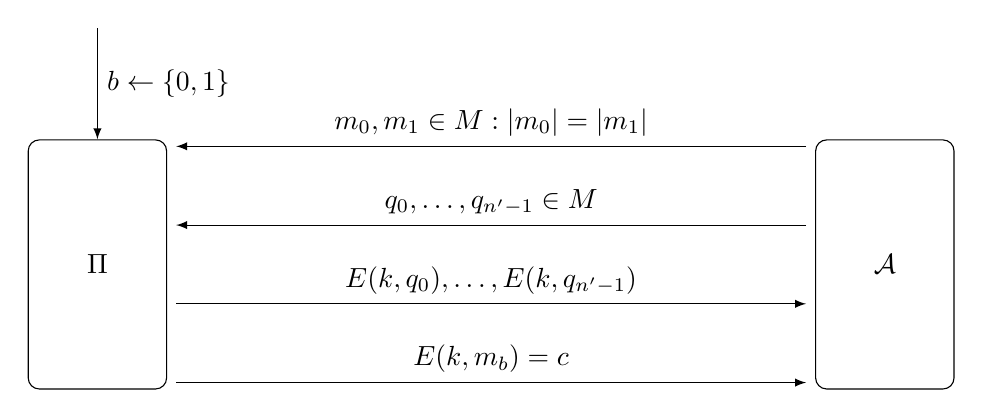
\begin{tikzpicture}[node distance=2cm,auto,>=latex]
\tikzset{
  player/.style={draw,shape=rectangle,rounded corners,minimum width=5em,minimum height=9em}
}
\node[player] (system) {$\Pi$};
\node[player] (adversary) at (10,0) {$\mathcal{A}$};
\draw[->] (9,1.5) -> node[above]{$m_0, m_1 \in M : |m_0| = |m_1|$} (1,1.5);
\draw[->] (9,0.5) -> node[above]{$q_0, \dots, q_{n'-1} \in M$} (1,0.5);
\draw[->] (1,-0.5) -> node[above]{$E(k, q_0), \dots, E(k, q_{n'-1})$} (9,-0.5);
\draw[->] (1,-1.5) -> node[above]{$E(k,m_b) = c$} (9,-1.5);
\draw[->] (0,3) -> node{$b \leftarrow \{0,1\}$} (system);
\end{tikzpicture}
\end{center}

Um sistema é {\em seguro contra CPA} se nenhum adversário polinomial tiver uma vantagem significativa para vencer o jogo que acabamos de descrever.
Ou seja, a probabilidade de que um adversário consiga vencer o jogo é apenas desprezivelmente maior do que $\frac{1}/{2}$

Para construir um sistema seguro contra ataques CPA, precisamos usar o conceito de funções pseudoaleatórias.
Em termos simples, uma função pseudoaleatória é um processo que transforma uma entrada (um conjunto de bits) em uma saída que parece aleatória.

A diferença principal é que a função pseudoaleatória não apenas estende ou gera uma sequência longa a partir de um pequeno pedaço de informação (como um gerador de números pseudoaleatórios faria), mas sim utiliza uma chave para definir a própria função que realiza essa transformação.
Em outras palavras, a chave é usada para escolher a função específica dentro de um grande conjunto de funções possíveis.
Quando aplicamos essa função a uma entrada, ela ``embaralha'' os bits de maneira que a saída pareça aleatória, mesmo sendo gerada de forma determinística.

A segurança de uma função pseudoaleatória é garantida pelo fato de que não existe um algoritmo eficiente (ou seja, que funcione em tempo polinomial) capaz de distinguir entre uma função pseudoaleatória e uma função escolhida de maneira verdadeiramente aleatória.
Em outras palavras, para qualquer adversário que tente diferenciar entre essas duas situações, a função pseudoaleatória será tão boa quanto uma função completamente aleatória.

Uma {\em cifra de bloco} é um tipo específico de função pseudoaleatória, que chamamos de {\em permutação pseudoaleatória}.
Sua característica distintiva é a capacidade de reverter o processo de ``embaralhamento'' dos bits.
Isso significa que, além de transformar uma mensagem de tamanho fixo (o {\em bloco}) em uma saída que parece aleatória, ela também permite que essa transformação seja desfeita de forma eficiente, recuperando a mensagem original.

Assim como outras funções pseudoaleatórias, a cifra de bloco utiliza uma chave para definir como os bits serão embaralhados.
A segurança dessa cifra vem do fato de que, para um adversário, ela é indistinguível de uma permutação completamente aleatória.
Ou seja, não existe um método eficiente para diferenciar entre o comportamento da cifra de bloco e o de uma função que simplesmente embaralha os bits de maneira aleatória.

Na próxima seção, veremos como essas cifras de bloco podem ser combinadas para criptografar mensagens de qualquer tamanho, mantendo a segurança do sistema criptográfico.

\section{Modos de Operação}
\label{sec:modos-de-operacao-bloco}

Uma cifra de bloco é usada para criptografar informações em pedaços de tamanho fixo, chamados de blocos.
No entanto, na prática, muitas vezes precisamos criptografar mensagens que são maiores ou menores que esse tamanho fixo.
Para lidar com isso, precisamos de uma forma de combinar os blocos criptografados pela cifra de bloco para proteger a mensagem inteira.

Uma maneira simples e intuitiva de fazer isso é chamada de {\em Electronic Code Book} (ECB).
Nesse modo de operação, dividimos a mensagem em vários blocos do mesmo tamanho e, em seguida, criptografamos cada um desses blocos separadamente com a cifra de bloco.
Depois de criptografar todos os blocos, simplesmente juntamos os blocos cifrados para formar a mensagem final cifrada.

No entanto, esse método tem uma grande falha de segurança:
blocos idênticos na mensagem original serão criptografados da mesma maneira, resultando em blocos idênticos no texto cifrado.
Isso significa que, se um adversário observar blocos repetidos no texto cifrado, ele pode deduzir que partes da mensagem original são iguais, o que compromete a segurança.

Por exemplo, imagine que um adversário queira descobrir se duas partes de uma mensagem criptografada são iguais ou diferentes.
Ele pode criar duas mensagens de teste:
uma onde a mesma parte se repete, e outra onde as duas partes são diferentes.

Se ele criptografar essas mensagens e o texto cifrado resultar em dois blocos idênticos, o adversário saberá que a mensagem original tinha partes iguais.
Se os blocos cifrados forem diferentes, ele saberá que as partes da mensagem original também eram diferentes.

Em outras palavras, esse adversário consegue distinguir entre as duas cifras ao observar como cada bloco é criptografado.
Isso significa que o modo ECB não é seguro nem mesmo contra ataques apenas contra a cifra.
A Figura \ref{fig:ecb-exemplo} ilustra essa vulnerabilidade.\footnote{Imagem tirada do verbete {\em Modo de Operação (criptografia)} da Wikipédia (\url{https://pt.wikipedia.org})}).

\begin{figure}[!htp]
  \label{fig:ecb-exemplo}
  \centering
  \includegraphics[width=.3\textwidth]{imagens/Tux.jpg}
  \includegraphics[width=.3\textwidth]{imagens/Tux_ecb.jpg}
  \caption{Imagem criptografada no modo ECB}
\end{figure}

Essa forma ingênua de combinar os blocos não garante a segurança contra os tipos de ataques mais básicos que discutimos anteriormente.
O que realmente precisamos é de um sistema que seja seguro contra ataques CPA, onde o adversário pode escolher mensagens e ver como elas são criptografadas.

Na definição de segurança contra CPA, o adversário tem a capacidade de ``consultar'' o sistema para descobrir como uma mensagem específica seria criptografada.
Isso significa que, para proteger o sistema, o processo de criptografia precisa ser imprevisível, ou seja, não pode produzir o mesmo resultado toda vez que a mesma mensagem é criptografada.
Se fosse previsível, o adversário poderia facilmente enganar o sistema ao enviar mensagens que ele já consultou antes.

Para garantir essa imprevisibilidade, incluímos um bloco aleatório no início de cada mensagem, conhecido como {\em vetor inicial} (IV).
Esse vetor inicial não precisa ser mantido em segredo, mas ele assegura que cada vez que uma mensagem é criptografada, o resultado será diferente, mesmo que a mensagem original seja a mesma.
Assim como nas cifras de fluxo, o vetor inicial é fundamental para evitar que padrões previsíveis apareçam no texto cifrado, aumentando a segurança do sistema.

No modo de operação {\em Encadeamento de Blocos de Cifra} ou {\em Cipher Block Chaining} (CBC), cada bloco de texto cifrado não depende apenas da cifra de bloco aplicada ao bloco de texto original, mas também do bloco cifrado que veio imediatamente antes dele.
Isso cria uma ``cadeia'' onde cada bloco cifrado influencia o próximo, aumentando a segurança do processo.

O funcionamento é o seguinte:

\begin{itemize}
\item Primeiro, temos um bloco aleatório inicial, o vetor inicial (IV), que inicia o processo ($c_0 = IV$).
  Esse bloco serve para garantir que cada mensagem cifrada será única.
\item Em seguida, cada bloco da mensagem original é combinado com o bloco cifrado anterior antes de ser criptografado ($p_k(c_{i-1} \xor m_i)$).
  Isso significa que, para criptografar um bloco da mensagem, usamos a cifra de bloco, mas também consideramos o resultado do bloco anterior.
\end{itemize}

Essa cadeia de dependência faz com que, mesmo que dois blocos da mensagem original sejam iguais, seus blocos cifrados finais sejam diferentes, porque cada um deles leva em conta o bloco anterior.
Ao final, o resultado é uma sequência de blocos cifrados, onde cada um depende do anterior, tornando o sistema muito mais seguro.

\begin{center}
\begin{tikzpicture}[node distance=2cm,auto,>=latex]
  \node (IVm) at (0,0)  {$IV$};
  \node (IVc) at (0,-3)  {$IV$};
  \node (m1) at (2,0)  {$m_1$};
  \node (xor1) at (2,-1)  {$\xor$};
  \node (c1) at (2,-3)  {$c_1$};
  \node (m2) at (4,0) {$m_2$};
  \node (xor2) at (4,-1)  {$\xor$};
  \node (c2) at (4,-3) {$c_2$};
  \node at (6,0) {\dots};
  \node at (6,-3) {\dots};
  \node (ml) at (8,0) {$m_l$};
  \node (xorl) at (8,-1)  {$\xor$};
  \node (cl) at (8,-3) {$c_l$};
  \draw[->] (IVm) -> (IVc);
  \draw[->] (IVc) -> (xor1);
  \draw[->] (m1) -> (xor1);
  \draw[->] (xor1) -> node[right]{$p_k$} (c1);
  \draw[->] (c1) -> (xor2);
  \draw[->] (m2) -> (xor2);
  \draw[->] (xor2) -> node[right]{$p_k$} (c2);
  \draw[->] (7,-1) -> (xorl);
  \draw[->] (ml) -> (xorl);
  \draw[->] (xorl) -> node[right]{$p_k$} (cl);
\end{tikzpicture}
\end{center}

Para descriptografar uma mensagem que foi cifrada usando o modo CBC, o processo é basicamente o inverso da criptografia.

Cada bloco da mensagem original é recuperado usando o bloco cifrado correspondente e o bloco cifrado anterior.
Em outras palavras, para descriptografar um bloco específico, aplicamos o processo inverso da cifra de bloco ao bloco cifrado seguinte e, em seguida, combinamos esse resultado com o bloco cifrado anterior ($m_{i}  :=  p_k^{-1}(c_{i+1}) \xor c_{i}$).

Esse processo continua ao longo de toda a sequência de blocos cifrados, revertendo o ``encadeamento'' até que todos os blocos da mensagem original tenham sido restaurados.

É possível provar que este sistema é seguro contra CPA.

\begin{theorem}
Um sistema que utiliza uma permutação pseudoaleatória segura no modo CBC é seguro contra ataques do tipo CPA.
\end{theorem}


A principal limitação do modo CBC é que os blocos de dados precisam ser processados em sequência, ou seja, cada bloco só pode ser criptografado depois que o bloco anterior foi processado.
Isso significa que o algoritmo não pode ser facilmente paralelizado, o que pode tornar o processo mais lento.

Por outro lado, o {\em modo contador} (Ctr) não tem essa limitação.
Esse modo funciona de maneira semelhante a uma cifra de fluxo, permitindo que os blocos sejam processados simultaneamente, o que aumenta a eficiência.

No modo Ctr, o processo começa com uma sequência de bits aleatória, o vetor inicial (IV), que é usado como ponto de partida.
Em vez de depender do bloco anterior, cada bloco da mensagem é combinado com um valor único, gerado ao somar o índice do bloco ao vetor inicial ($IV + i$).
Esse valor é então processado por uma função pseudoaleatória, e o resultado é combinado com o bloco da mensagem para produzir o texto cifrado ($c_i = m_i \xor f_k(IV + i)$).

\begin{center}
\begin{tikzpicture}[node distance=2cm,auto,>=latex]
  \node (IVm) at (0,0)  {$IV$};
  \node (IVc) at (0,-3)  {$IV$};
  \node (IV1) at (2,0)  {$IV + 1$};
  \node (xor1) at (2,-2)  {$\xor$};
  \node (c1) at (2,-3)  {$c_1$};
  \node (IV2) at (4,0) {$IV + 2$};
  \node (xor2) at (4,-2)  {$\xor$};
  \node (c2) at (4,-3) {$c_2$};
  \node at (6,0) {\dots};
  \node at (6,-3) {\dots};
  \node (IVl) at (8,0) {$IV + l$};
  \node (xorl) at (8,-2)  {$\xor$};
  \node (cl) at (8,-3) {$c_l$};
  \draw[->] (IVm) -> (IVc);
  \draw[->] (1,-2) -> node[above]{$m_1$} (xor1);
  \draw[->] (IV1) -> node[right]{$f_k$} (xor1);
  \draw[->] (xor1) ->  (c1);
  \draw[->] (3,-2) -> node[above]{$m_2$} (xor2);
  \draw[->] (IV2) -> node[right]{$f_k$} (xor2);
  \draw[->] (xor2) ->  (c2);
  \draw[->] (7,-2) -> node[above]{$m_l$} (xorl);
  \draw[->] (IVl) -> node[right]{$f_k$} (xorl);
  \draw[->] (xorl) -> (cl);
\end{tikzpicture}
\end{center}

Para descriptografar uma mensagem no modo contador (Ctr), o processo é simples e eficiente.
Primeiro, somamos o vetor inicial (IV) ao número do bloco que estamos tentando recuperar.
Em seguida, aplicamos a mesma função usada durante a criptografia para gerar o bloco de bits correspondente e, por fim, realizamos a operação XOR entre essa sequência e o bloco cifrado correspondente ($c_i \xor f_k(IV + i)$).

Ao contrário do modo CBC, não precisamos reverter a função utilizada na criptografia.
Em outras palavras, não é necessário usar uma permutação pseudoaleatória que permita desfazer o processo de ``embaralhamento''.
Uma função simples que embaralha os bits de maneira segura é suficiente para tanto a criptografia quanto a descriptografia.

O modo Ctr também é seguro contra ataques do tipo CPA.

\begin{theorem}
Um sistema que utiliza uma função pseudoaleatória segura no modo Ctr é seguro contra ataques do tipo CPA.
\end{theorem}

Para se convencer de que o teorema é válido, vamos considerar dois sistemas de criptografia:
o sistema $\Pi$, que usa uma função pseudoaleatória no modo contador (Ctr), e o sistema $\Pi'$, que é semelhante, mas usa uma função realmente aleatória.

Suponha que exista um adversário $\mathcal{A}$ que tenta atacar o sistema.
Para analisar a segurança, podemos imaginar que estamos tentando construir um distinguidor que tenta identificar se o sistema está usando uma função pseudoaleatória ou uma função realmente aleatória.

O processo seria o seguinte:

\begin{enumerate}
\item Sempre que o adversário $\mathcal{A}$ quiser saber como uma mensagem seria criptografada, geramos um vetor inicial (IV) e, em seguida, aplicamos a função (seja ela pseudoaleatória ou realmente aleatória) ao vetor inicial somado ao número do bloco correspondente.
  O resultado é então combinado com a mensagem original para gerar o texto cifrado que é devolvido ao adversário.
\item Quando o adversário $\mathcal{A}$ tenta adivinhar entre duas mensagens enviadas ao sistema, o processo é o mesmo:
  geramos um vetor inicial, aplicamos a função escolhida e combinamos o resultado com as mensagens que o adversário deseja testar.
\end{enumerate}

Se o sistema $\Pi'$ usa uma função realmente aleatória, ele se comporta como uma ``caixa preta'' que não permite que o adversário aprenda nada útil sobre a mensagem original, além do que poderia descobrir por simples adivinhação.
Neste caso, a chance de sucesso do adversário é equivalente a um palpite aleatório ($50\%$).

Agora, precisamos verificar se o sistema $\Pi$, que usa uma função pseudoaleatória, se comporta de maneira suficientemente semelhante ao sistema $\Pi'$ para que o adversário não possa distinguir entre eles.
Se a função pseudoaleatória usada for segura, ela será praticamente indistinguível de uma função realmente aleatória, o que significa que a chance do adversário distinguir entre as duas será desprezivelmente superior a $\frac{1}{2}$.

A única maneira de o adversário ganhar uma vantagem é se o vetor inicial usado para criptografar coincider com o da mensagem que ele está testando.
No entanto, como o número total de possibilidades para o vetor inicial é enorme ($2^n$ para um bloco de tamanho $n$), a probabilidade de tal coincidência ocorrer é desprezível.

Portanto, a chance do adversário ter sucesso em um ataque CPA contra o sistema $\Pi$ é apenas desprezivelmente superior a $\frac{1}{2}$.
Isso nos permite concluir que o sistema $\Pi$ é seguro contra ataques CPA.

A explicação indica que o tamanho dos blocos também influencia em sua segurança.
Isso ocorre, pois quanto menores os blocos maior a chance de gerar vetores inciais idênticos, e portanto, de criptografar duas mensagens distintas com a mesma chave.

\section{Construções Práticas}
\label{sec:construcoes-praticas}

Como vimos anteriormente, uma Permutação Pseudoaleatória (PRP) é um método que embaralha blocos de dados de forma que o resultado final seja imprevisível.
Essa permutação é gerada de maneira determinística, ou seja, segue um processo definido a partir de uma chave específica.

A segurança de uma permutação pseudoaleatória depende de dois fatores principais:
o tamanho da chave usada para gerar a permutação e o tamanho dos blocos de dados que estão sendo embaralhados.
Quanto maiores forem esses parâmetros, mais difícil será para alguém sem a chave prever ou decifrar a permutação utilizada.

Imaginemos que temos uma chave aleatória e uma função que, a partir dessa chave, cria uma permutação dos dados.
O objetivo é que essa permutação seja indistinguível de uma permutação completamente aleatória, mesmo para quem está tentando analisar o sistema de fora.
Embora não conheçamos um sistema comprovadamente seguro em termos de ser totalmente aleatório, na prática, sistemas como o AES (Advanced Encryption Standard) têm se mostrado eficazes e seguros.

O desafio aqui é desenvolver um algoritmo onde, ao mudar um único bit, seja na chave ou na mensagem, isso tenha um impacto significativo em toda a cifra resultante.
Isso significa que uma pequena alteração deve se espalhar por toda a saída, dificultando a previsibilidade do resultado.

Para alcançar esse efeito, utilizamos o conceito de confusão e difusão, proposto por Claude Shannon, um dos pioneiros na teoria da criptografia \cite{Shannon49}.
A {\em confusão} é a técnica de tornar a relação entre a chave e o texto cifrado tão complexa quanto possível.
Um exemplo simples é dividir o bloco de dados em pedaços menores, como grupos de 8 bits, e substituí-los por novos valores, seguindo uma tabela de substituição.
Entretanto, apenas confundir os dados não é suficiente.
Se alterarmos um bit no início do processo, isso pode afetar apenas uma pequena parte do resultado final.

É aí que entra a {\em difusão}, que tem como objetivo espalhar a influência dessa pequena mudança por todo o bloco de dados.
Em cifras de bloco modernas, essas fases de confusão e difusão são repetidas várias vezes para garantir que qualquer pequena alteração na entrada cause uma mudança ampla e complexa na saída.


\subsection{Data Encryption Standard (DES)}
\label{sec:des}

O {\em Data Encryption Standard} (DES) foi o padrão de criptografia para cifras de bloco que predominou do final dos anos 1970 até o final dos anos 1990.
Esse algoritmo foi originalmente desenvolvido pela IBM, mas passou por modificações significativas feitas pela NSA (Agência de Segurança Nacional dos Estados Unidos) antes de se tornar um padrão internacional.

O DES utiliza uma estrutura conhecida como {\em rede de Feistel}, que permite a criação de uma função criptográfica que pode ser invertida de forma eficiente.
Esse tipo de rede funciona aplicando uma série de funções sobre os dados de entrada, o que facilita a criptografia e a descriptografia.

Quando o DES processa uma mensagem, essa mensagem é dividida em duas partes iguais.
Vamos chamar essas partes de $L$ (a primeira metade) e $R$ (a segunda metade).
Em cada etapa do processo de criptografia, essas partes são manipuladas da seguinte maneira:
\begin{itemize}
\item $L$ se torna igual a $R$ da etapa anterior.
\item $R$ se torna igual ao valor de $L$ da etapa anterior, combinado com o resultado da função aplicada em $R$.
  \begin{displaymath}
    L_i := R_{i-1} \textrm{ e } R_i := L_{i-1} \xor f_i(R_{i-1})
  \end{displaymath}
\end{itemize}

Esse processo é repetido várias vezes, o que garante que até mesmo pequenas alterações na entrada resultem em grandes mudanças na saída criptografada, tornando o sistema mais seguro e difícil de ser quebrado.


\begin{center}
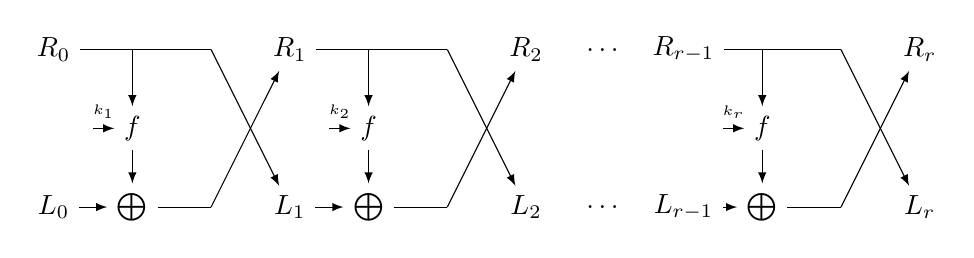
\begin{tikzpicture}[node distance=2cm,auto,>=latex]
  \node (R0) at (0,0)  {$R_0$};
  \node (L0) at (0,-2)  {$L_0$};
  \node (F0) at (1,-1)  {$f$};
  \node (xor0) at (1,-2)  {$\bigoplus$};
  \node (R1) at (3,0)  {$R_1$};
  \node (L1) at (3,-2)  {$L_1$};
  \node (F1) at (4,-1) {$f$};
  \node (xor1) at (4,-2)  {$\bigoplus$};
  \node (R2) at (6,0)  {$R_2$};
  \node (L2) at (6,-2) {$L_2$};
  \node at (7,0) {\dots};
  \node at (7,-2) {\dots};
  \node (Rr1) at (8,0) {$R_{r-1}$};
  \node (Lr1) at (8,-2)  {$L_{r-1}$};
  \node (Fr) at (9,-1) {$f$};
  \node (xorr) at (9,-2)  {$\bigoplus$};
  \node (Rr) at (11,0) {$R_{r}$};
  \node (Lr) at (11,-2)  {$L_{r}$};

  \draw[-] (R0) -> (2,0);
  \draw[->] (1,0) -> (F0);
  \draw[->] (L0) -> (xor0);
  \draw[->] (0.5,-1) -> node[above]{\tiny{$k_1$}} (F0);
  \draw[->] (F0) -> (xor0);
  \draw[-] (xor0) -> (2,-2);
  \draw[->] (2,0) -> (L1);
  \draw[->] (2,-2) -> (R1);

  \draw[-] (R1) -> (5,0);
  \draw[->] (4,0) -> (F1);
  \draw[->] (L1) -> (xor1);
  \draw[->] (3.5,-1) -> node[above]{\tiny{$k_2$}} (F1);
  \draw[->] (F1) -> (xor1);
  \draw[-] (xor1) -> (5,-2);
  \draw[->] (5,0) -> (L2);
  \draw[->] (5,-2) -> (R2);

  \draw[-] (Rr1) -> (10,0);
  \draw[->] (9,0) -> (Fr);
  \draw[->] (Lr1) -> (xorr);
  \draw[->] (8.5,-1) -> node[above]{\tiny{$k_r$}} (Fr);
  \draw[->] (Fr) -> (xorr);
  \draw[-] (xorr) -> (10,-2);
  \draw[->] (10,0) -> (Lr);
  \draw[->] (10,-2) -> (Rr);
\end{tikzpicture}
\end{center}

Quando trabalhamos com uma rede de Feistel, podemos facilmente reverter o processo de criptografia para recuperar os dados originais.
Suponha que estamos na $i$-ésima rodada da rede e que temos as saídas $L_i$ e $R_i$ dessa rodada.
Para recuperar os valores da rodada anterior, $L_{i-1}$ e $R_{i-1}$, seguimos um processo simples:

\begin{itemize}
\item Primeiro, definimos $R_{i-1}$ como igual a $L_i$.
  Isso porque, em uma rede de Feistel, $L_i$ sempre vem diretamente de $R$ da rodada anterior.
\item Depois, calculamos $L_{i-1}$ pegando o valor atual de $R_i$ e combinando-o com o resultado da função aplicada em $R_{i-1}$.

  \begin{displaymath}
    L_{i-1} := R_i \xor f_i(R_{i-1})
  \end{displaymath}
\end{itemize}

Ao repetir esse procedimento para cada rodada, conseguimos inverter todo o processo de criptografia, retornando à mensagem original.

O \textit{Data Encryption Standard} (DES) é um algoritmo de criptografia que utiliza uma estrutura chamada rede de Feistel com 16 etapas (ou rodadas).
Ele trabalha com blocos de dados de 64 bits e utiliza uma chave de 64 bits para a criptografia.
No entanto, desses 64 bits, apenas 56 são efetivamente utilizados para a criptografia, pois 8 bits são descartados logo no início do processo.
Assim, o DES é descrito como uma função que combina uma chave de 56 bits com um bloco de 64 bits de dados para produzir um novo bloco criptografado de 64 bits, ou seja, $DES: \{0,1\}^{56} \times \{0,1\}^{64} \to \{0,1\}^{64}$.

A chave de 56 bits passa por um processo chamado \textit{key schedule}, que gera 16 subchaves, cada uma com 48 bits, para serem usadas em cada uma das 16 rodadas de criptografia.

Em cada rodada do DES, a mesma função é aplicada.
Essa função recebe uma subchave de 48 bits e metade do bloco de 64 bits (ou seja, 32 bits) como entrada, e produz uma nova sequência de 32 bits como saída.
Aqui está como essa função funciona:

\begin{enumerate}
    \item {\em Expansão}: Primeiro, os 32 bits do bloco são expandidos para 48 bits,
    \item {\em XOR}: Esses 48 bits são combinados com a subchave utilizando a operação XOR (ou \textit{ou exclusivo}), que mistura os bits de uma forma difícil de reverter sem a chave correta,
    \item {\em Divisão}: O resultado é então dividido em 8 partes, cada uma com 6 bits,
    \item {\em S-Boxes}: Cada uma dessas partes de 6 bits passa por uma substituição através de uma tabela especial chamada \textit{SBox}, que reduz os 6 bits para 4 bits.
      Essa é a fase de \textit{confusão}, que torna a relação entre a chave e a saída bem complexa,
    \item {\em Redução}: Após essa substituição, os 8 grupos de 4 bits são combinados de volta em uma sequência de 32 bits,
    \item {\em Difusão}: Finalmente, esses 32 bits são embaralhados em um processo chamado \textit{difusão}, que espalha as mudanças por todo o bloco, garantindo que até mesmo pequenas alterações na entrada resultem em grandes mudanças na saída.
\end{enumerate}


\begin{figure}[!htp]
  \centering
  \includegraphics[width=.4\textwidth]{imagens/feistel-function.png}
  \caption{Função de Fiestel do DES}
  \label{fig:feistel-function}
\end{figure}

A adoção do DES como padrão de criptografia não foi isenta de controvérsias.
Um dos pontos mais discutidos foi o descarte de 8 bits da chave original de 64 bits, reduzindo-a para 56 bits sem uma justificativa clara.
Na época, uma chave de 56 bits estava no limite da segurança, mas hoje sabemos que ela é vulnerável a ataques de força bruta.

Além do pequeno tamanho da chave, outro aspecto suspeito foi a modificação das S-Boxes pela NSA (Agência de Segurança Nacional dos Estados Unidos) sem grandes explicações antes que o algoritmo fosse adotado como padrão.
Anos mais tarde, pesquisadores apresentaram uma técnica chamada {\em criptoanálise diferencial}, que tornou várias cifras inseguras.
No entanto, surpreendentemente, o DES resistiu a essa técnica.
Isso levou à suspeita de que os pesquisadores da NSA já conheciam a criptoanálise diferencial e ajustaram o DES de forma que ele se tornasse seguro contra esse tipo de ataque.

Em 1993, um artigo já alertava para a fragilidade dessa chave, propondo um projeto de hardware que, teoricamente, seria capaz de quebrar uma chave de 56 bits em apenas um dia e meio.
Essa previsão se tornou realidade em 1998, quando a {\em Electronic Frontier Foundation} (EFF)  — uma organização sem fins lucrativos que defende a privacidade, a liberdade de expressão e os direitos digitais na internet — construiu uma máquina chamada Deep Crack.
Este dispositivo, que custou cerca de 250 mil dólares, conseguiu quebrar uma cifra DES em 56 horas, aproximadamente dois dias e meio.

A situação se agravou ainda mais em 2006, quando pesquisadores alemães desenvolveram um hardware de baixo custo — em torno de 10 mil dólares — capaz de realizar um ataque de força bruta ao DES em menos de uma semana.
Essa evolução mostra que, enquanto nos anos 80 apenas grandes potências mundiais tinham os recursos para construir máquinas desse tipo, hoje em dia, qualquer entidade com recursos relativamente modestos pode quebrar o DES.

Com essas revelações e avanços, o DES, que antes era o padrão de segurança, é agora considerado totalmente inseguro para proteger informações sensíveis.

\subsection{Advanced Encryption Standard (AES)}
\label{sec:aes}

As crescentes preocupações em torno da segurança do DES, especialmente devido à possibilidade iminente de ataques de força bruta contra sua chave de 56 bits, levaram o NIST (Instituto Nacional de Padrões e Tecnologia dos Estados Unidos) a buscar uma solução mais segura.
Em 1997, o NIST organizou um concurso acadêmico internacional para desenvolver um novo padrão de criptografia que pudesse substituir o DES.

Este concurso, chamado Advanced Encryption Standard (AES) Competition, incentivou pesquisadores e criptógrafos de todo o mundo a submeterem seus algoritmos de criptografia.
Além de criar e apresentar um algoritmo, cada participante também tinha a tarefa de analisar e encontrar possíveis vulnerabilidades nos algoritmos dos outros concorrentes.
Isso ajudou a garantir que o novo padrão fosse robusto e resistente a ataques.

Após uma rigorosa avaliação, cinco algoritmos finalistas foram considerados adequados para se tornarem o novo padrão de criptografia.
Em abril de 2000, o algoritmo {\em Rijndael} foi anunciado como o vencedor do concurso.
Este algoritmo, desenvolvido por dois criptógrafos belgas, foi então adotado como o novo padrão de criptografia e recebeu o nome de AES ({\em Advanced Encryption Standard}).
Desde então, o AES tem sido amplamente utilizado e é considerado um dos algoritmos de criptografia mais seguros disponíveis atualmente.

O \textit{AES} é um algoritmo de criptografia que opera em blocos de 128 bits.
Ele possui três versões, cada uma utilizando um tamanho de chave diferente e um número correspondente de rodadas de criptografia:

\begin{itemize}
    \item \textbf{AES-128}: Usa chaves de 128 bits e realiza 10 rodadas de criptografia.
    \item \textbf{AES-192}: Usa chaves de 192 bits e realiza 12 rodadas de criptografia.
    \item \textbf{AES-256}: Usa chaves de 256 bits e realiza 14 rodadas de criptografia.
\end{itemize}

Ao contrário do \textit{DES}, que utiliza uma estrutura chamada \textit{rede de Feistel} para sua criptografia, o AES adota uma técnica diferente, conhecida como \textit{rede de substituição e permutação}.
Essa técnica envolve a substituição de dados em cada rodada seguida por uma permutação, ou rearranjo, dos bits, o que contribui para a robustez e a segurança do algoritmo.

No \textit{AES}, o bloco de dados a ser criptografado é inicialmente dividido em 8 sequências de 16 bits. Essas sequências são organizadas em uma estrutura conhecida como \textit{estado}, que é representada por uma matriz 4x4, onde cada célula da matriz corresponde a um bloco de 8 bits.

Durante o processo de criptografia, o AES realiza várias rodadas, onde em cada rodada o algoritmo aplica uma série de transformações ao estado.
As transformações em cada rodada são as seguintes (conforme ilustrado na Figura \ref{fig:aes}):

\begin{enumerate}
\item \textbf{AddRoundKey:} O primeiro passo de cada rodada é adicionar uma subchave ao estado.
  A subchave é gerada pelo processo de \textit{key schedule} do AES, que produz uma subchave de 128 bits para cada rodada.
  Essa subchave é combinada com o estado usando a operação XOR, que mistura os bits da chave com os bits do estado de maneira que apenas quem possui a chave correta possa decifrar o bloco.

\item \textbf{SubBytes:} No segundo passo, cada byte do estado é substituído por um novo byte.
  Essa substituição é feita usando uma tabela de substituição chamada \textit{SBox}, que é bijetora, ou seja, cada entrada tem uma saída única e distinta.
  Esse passo, conhecido como fase de confusão, tem como objetivo dificultar a relação direta entre o texto original e o texto criptografado.

\item \textbf{ShiftRows:} Em seguida, ocorre a etapa de \textit{ShiftRows}, onde as linhas da matriz são rotacionadas.
  A primeira linha permanece inalterada, enquanto a segunda linha é rotacionada uma posição para a esquerda, a terceira linha duas posições, e a quarta linha três posições.
  Essa etapa contribui para espalhar os bytes ao longo do estado, aumentando a complexidade da criptografia.

\item \textbf{MixColumns:} Por fim, a etapa \textit{MixColumns} trata as quatro colunas do estado como vetores e as multiplica por uma matriz fixa específica.
  Essa operação garante que a alteração de qualquer byte de entrada afete múltiplos bytes de saída, promovendo o efeito de difusão, onde as mudanças nos dados de entrada se propagam amplamente pelo bloco criptografado.
\end{enumerate}

Esses quatro passos são repetidos em cada rodada do AES, contribuindo para a robustez e a segurança do algoritmo.

Na última rodada do \textit{AES}, a etapa de \textit{MixColumns} é substituída por uma segunda aplicação da fase \textit{AddRoundKey}.
Essa mudança finaliza o processo de criptografia de maneira segura e garante que a transformação aplicada ao estado seja adequadamente embaralhada antes de ser enviada como saída.

O AES foi cuidadosamente projetado para ser eficientemente reversível, mas apenas quando se tem a chave correta.
Isso significa que, com a chave, é possível decifrar os dados criptografados de forma rápida e precisa, o que é essencial para a segurança e a utilidade prática do algoritmo.

Até a escrita destas notas, não há conhecimento de um ataque contra o AES que seja mais eficiente do que o ataque de força bruta.
Em outras palavras, a única maneira conhecida de quebrar a criptografia do AES seria testar todas as chaves possíveis, o que, devido ao tamanho das chaves usadas pelo AES, é computacionalmente inviável com a tecnologia atual.


\begin{figure}[!htp]
  \centering
  \begin{minipage}{.45\textwidth}
    \centering
    \includegraphics[width=\textwidth]{imagens/AddRoundKey.png}  
  \end{minipage}
 \begin{minipage}{.45\textwidth}
    \centering
    \includegraphics[width=\textwidth]{imagens/SubBytes.png}
  \end{minipage}
  \begin{minipage}{.45\textwidth}
    \centering
    \includegraphics[width=\textwidth]{imagens/ShiftRows.png}  
  \end{minipage}
 \begin{minipage}{.45\textwidth}
    \centering
    \includegraphics[width=\textwidth]{imagens/MixColumns.png}
  \end{minipage}
  \caption{Etapas do AES}
  \label{fig:aes}
\end{figure}



\section{Exercícios}
\label{sec:exercicios}

\begin{exercicio}
  Considere a definição de segurança contra CPA em que consideramos qualquer adversário $\mathcal{A}$ -- não apenas os eficientes -- e exigimos que $Pr[PrivK^{cpa}_{\Pi,\mathcal{A}}(n) = 1] = \frac{1}{2}$.
  Mostre que é impossível construir um sistema que satisfaça essa definição de segurança.
\end{exercicio}

\begin{exercicio}
Mostre que a operação $R_i \xor f_i(R_{i-1})$ na rede de Feistel de fato recupera o valor de $L_{i-1}$.
\end{exercicio}

\begin{exercicio}
  Mostre que os modos CBC e Ctr são corretos, ou seja, que em ambos os casos $D(k, E(k,m)) = m$;
\end{exercicio}

\begin{exercicio}
  Suponha que $f$ seja uma função pseudo-aleatória com chave e blocos ambos de 128 bits e considere o seguinte sistema:
  \begin{enumerate}
  \item Seleciona aleatoriamente duas sequência de 128 bits, a chave $k$ e o vetor inicial $IV$
  \item Divide a mensagem $m$ em blocos de 128 bits: $m_0, m_1, \dots, m_{n-1}$ (podemos supor que $|m|$ é múltiplo de 128).
  \item A cifra $c = c_0 || c_1 || \dots || c_{n-1}$ é tal que $c_i = m_i \oplus f_k(IV)$ para $i = 0, ..., n-1$
  \item Para descriptografar fazemos $c_i \oplus f_k(IV)$ para $i = 0, \dots, n-1$.
  \end{enumerate}
  Esse sistema é seguro? Por que?
\end{exercicio}

\begin{exercicio}
Suponha que um bit em uma cifra tenha sido alterado por um erro.
Qual o efeito disso na mensagem descriptografada caso a cifra tenha sido produzida usando o modo Ctr? E no caso de ter sido produzida usando o modo CBC?  
\end{exercicio}



